\begin{figure}
    \begin{center}
    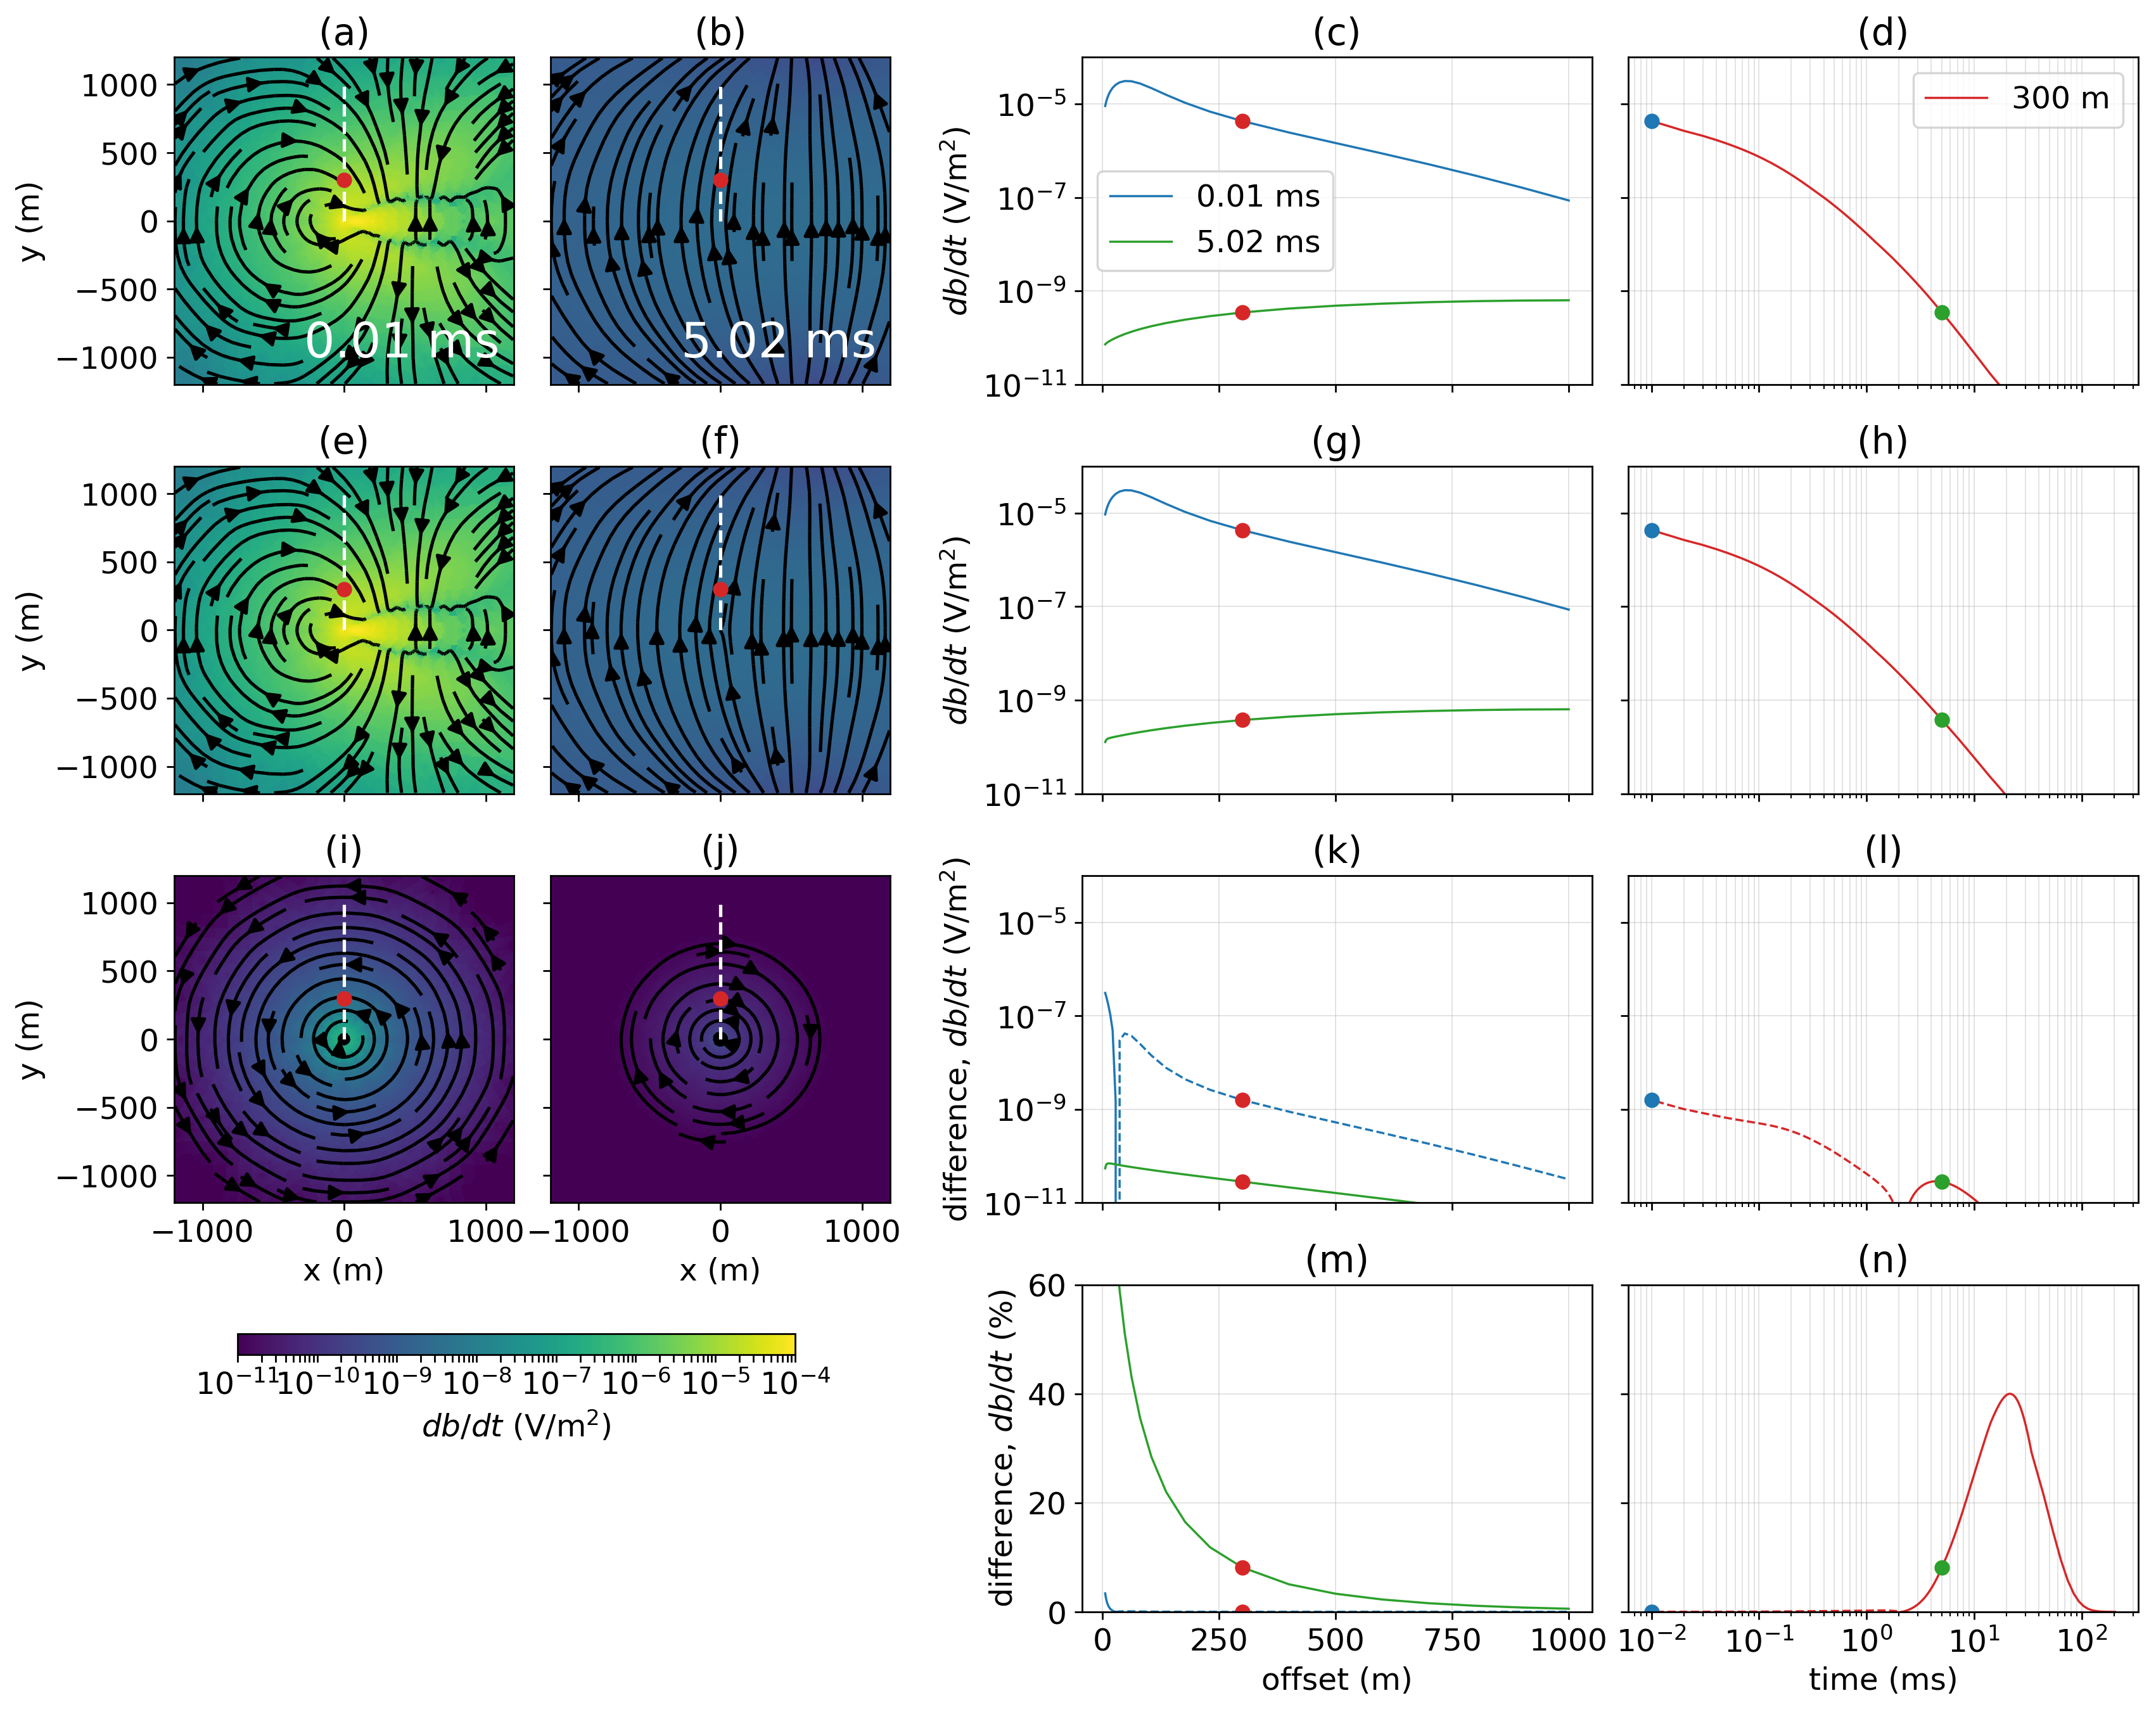
\includegraphics[width=\textwidth]{figures/em_casing/surface_dbdt_permeable.png}
    \end{center}
\caption{
    Simulated $db/dt$ at the surface of the earth, as was presented in \ref{fig:surface_dbdt_overview}.
    The top row (a -- d) are the data simulated with the conductive casing. The second rows (e -- h) are the data
    simulated with the conductive, permeable casing. The third row (i -- l) is the difference (permeable and conductive minus conductive only),
    and the fourth row (m and n) show the difference as a percentage of the conductive solution.
}
\label{fig:surface_dbdt_permeable}
\end{figure}



